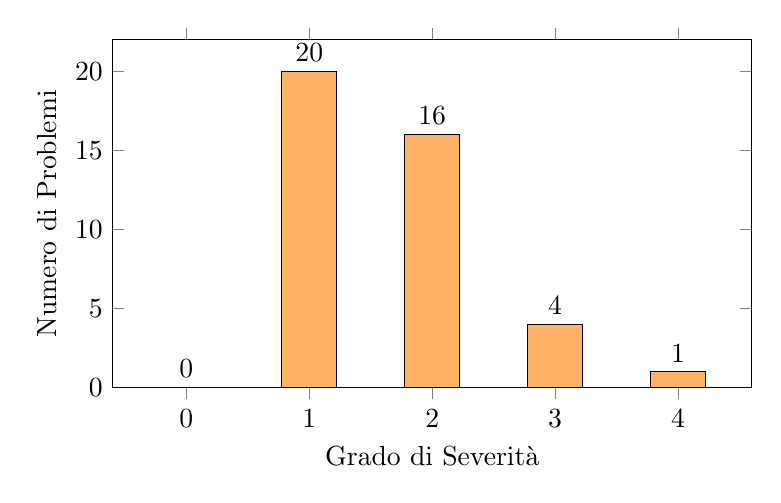
\begin{tikzpicture}
    \begin{axis}[
        ybar,
        bar width=20pt,
        enlarge x limits=0.15,
        ylabel={Numero di Problemi},
        xlabel={Grado di Severità},
        symbolic x coords={0, 1, 2, 3, 4},
        xtick=data,
        nodes near coords,
        nodes near coords align={vertical},
        width=0.8\textwidth,
        height=6cm,
        ymin=0
    ]
        \addplot[fill=orange!60] coordinates { (0,0) (1,20) (2,16) (3,4) (4,1) };
    \end{axis}
\end{tikzpicture}